\documentclass{standalone}

\usepackage{tikz}
     \usetikzlibrary{arrows.meta}   
\usepackage{graphicx} % Работа с графикой \includegraphics{}
\graphicspath{{./images/img1/}} % картинки в папке ./images/img1/
    
\begin{document}

\begin{tikzpicture}
    \node at (0,0) 
        {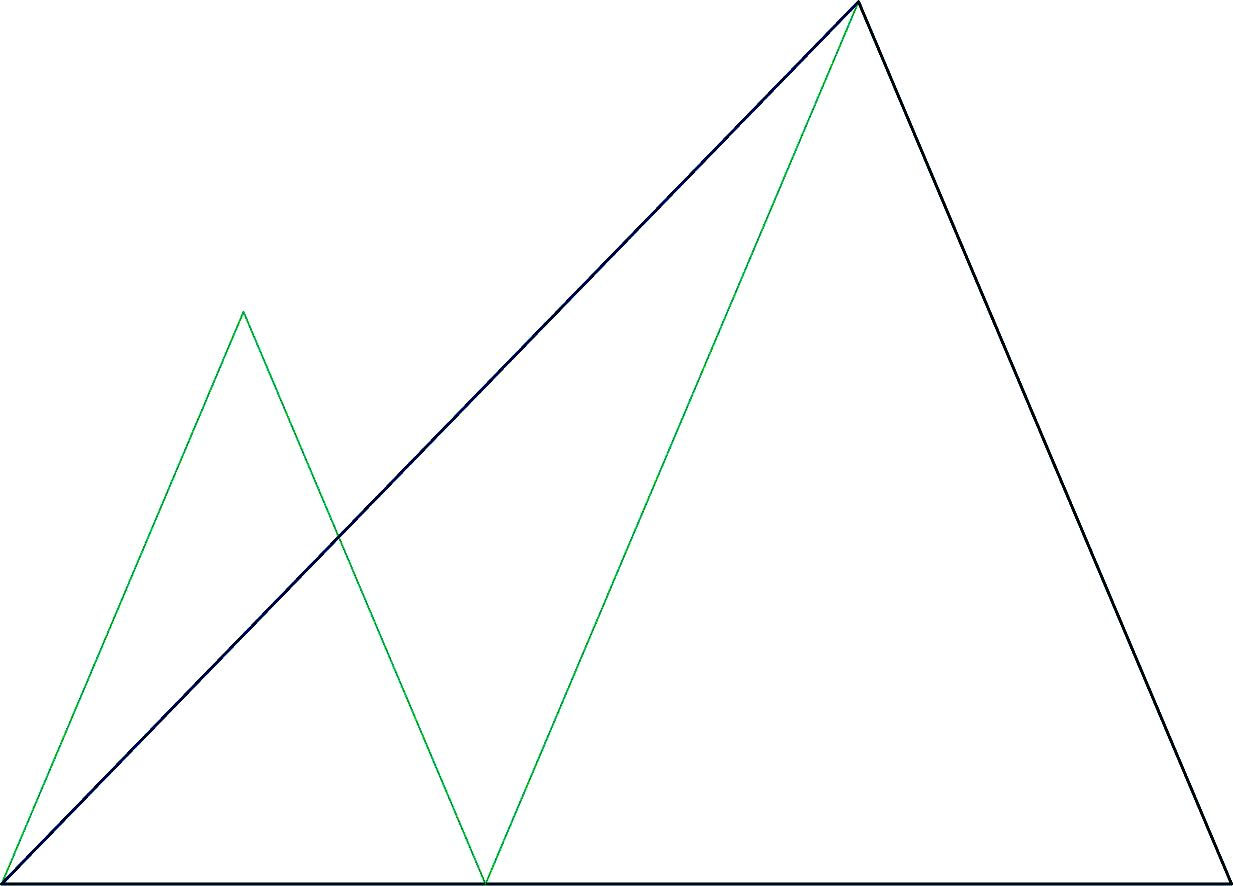
\includegraphics[width=4cm]{gps1.jpg}};
    \node[left] at (-2,-1.4) {$1$};
    \node[right] at (2,-1.4) {$2$};
    \node at (0.8,1.7) {$3$};
    \node[blue] at (-1.7,-1.3) {\small $2$};
    \node[blue] at (-0.7,-1.3) {\small $3$};
    \node[blue] at (-1.2,0.1) {\small $1$};
    \node[red] at (-0.2,-1.3) {\small $2$};
    \node[red] at (1.7,-1.3) {\small $3$};
    \node[red] at (0.8,1.1) {\small $1$};
    \node[blue] at (-1.1,-0.9) {$P_1$};
    \node[red] at (.8,0) {$P_2$};
    \node[shape=circle, draw] (a1) at ( 4,-1.3) {$1$};
    \node[shape=circle, draw] (a2) at ( 8,-1.3) {$2$};
    \node[shape=circle, draw] (a3) at ( 6,1.5)  {$3$};
    \path[->,>={Latex[length=8pt]}] 
        (a1) edge node[blue, above]{\bf 1}      (a2)
        (a2) edge node[red, above right]{\bf 2} (a3)
        (a3) edge node[red, above left]{\bf 2}  (a1);
\end{tikzpicture}

\end{document}